\chapter{SWID Generator}

\section{Requirements}

\subsection{Zweck}

Der SWID Generator soll ein kleines Programm für Linux-Systeme sein, welches aus
den Informationen in Paket Management Systemen SWID Tags generiert.

\subsection{Nichtfunktionale Anforderungen}

\begin{itemize}
		\item Als Implementationsprache wird Python verwendet.
		\item Es sollen möglichst wenig Abhängigkeiten zu Drittkomponenten wie
			Libraries/Frameworks entstehen.
    \item Die Software soll einfach zu installieren sein, beispielsweise durch
			Upload in den Python Package Index ($\rightarrow$ \texttt{pip install
			swid-generator}) oder durch Erstellen von \texttt{.deb}- und
			\texttt{.rpm}-Paketen.
		\item Als Quelle der Paketinformationen sollen Paketmanager wie DPKG und RPM
			verwendet werden.
\end{itemize}

\subsection{Use Cases}

Nachfolgend sind sind die identifizierten Use Cases für die Client Komponenten
des SWID-Generator aufgeführt.

Dabei werden die folgen drei Systemkomponenten berücksichtigt, welche
gegenseitig über die Standardeingabe und -ausgabe kommunizieren.

\vspace{1em}

\begin{figure}[H]
	\centering
	\definecolor{StrongswanColor}{RGB}{199,108,107}
\definecolor{GeneratorColor}{RGB}{116,143,204}
\definecolor{PkgMgrColor}{RGB}{227,225,107}

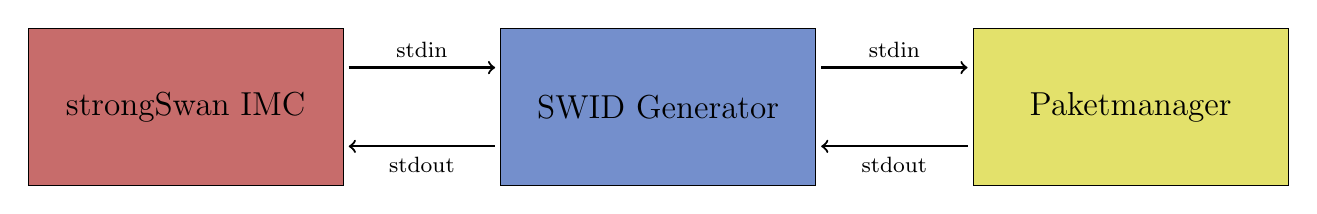
\begin{tikzpicture}[
		actor/.style={font=\large},
		communication/.style={thick, shorten <= 2pt, shorten >= 2pt, font=\footnotesize}
	]

	% Rectangles
	\filldraw[fill=StrongswanColor] (0, 0) rectangle node[actor] {strongSwan IMC} (4, 2);
	\filldraw[fill=GeneratorColor] (6, 0) rectangle node[actor] {SWID Generator} (10, 2);
	\filldraw[fill=PkgMgrColor] (12, 0) rectangle node[actor] {Paketmanager} (16, 2);

	% Arrows
	\draw[->, communication] (4, 1.5) -- node[above] {stdin} (6, 1.5);
	\draw[<-, communication] (4, 0.5) -- node[below] {stdout} (6, 0.5);
	\draw[->, communication] (10, 1.5) -- node[above] {stdin} (12, 1.5);
	\draw[<-, communication] (10, 0.5) -- node[below] {stdout} (12, 0.5);


\end{tikzpicture}

	\caption{SWID Generator: Systemkomponenten}
	\label{img:swid-generator-aktoren}
\end{figure}

\subsubsection{UC01: Erkennung des Paketmanagers}

\begin{usecase}
\hline
\textbf{Akteur} & strongSwan IMC \\
\hline
\textbf{Story} &
Der Akteur weiss nicht welcher Paketmanager auf dem Zielsystem verwendet wird.
Der SWID Generator soll den verwendeten Paketmanager automatisch erkennen. \\
\hline
\textbf{Standard Szenario} &
Der SWID Generator erkennt den System-Paketmanager automatisch. \\
\hline
\textbf{Alternatives Szenario} &
Mittels optionalem Parameter kann der zu verwendende Paketmanager definiert
werden, die automatische Erkennung wird dadurch übersteuert. \\
\hline
\end{usecase}


\subsubsection{UC02: Software ID Generierung}

\begin{usecase}
\hline
\textbf{Akteur} & strongSwan IMC \\
\hline
\textbf{Story} &
Der Akteur will Software IDs aller installierten Pakete generieren. Das Format
dieser IDs folgt dem ISO Draft 19770-2-5 \cite{iso19770-2-5} und besteht
aus der Regid des Tag Creators sowie der Unique ID des Tags. \\
\hline
\textbf{Standard Szenario} &
Alle Software IDs werden generiert und auf der Standardausgabe durch Newlines
(\texttt{\textbackslash{n}}) getrennt ausgegeben. Es wird eine Software ID pro Zeile
ausgegeben. \\
\hline
\textbf{Alternatives Szenario} &
Die Trennzeichen zur Ausgabe der Software IDs können mittels optionalem
Parameter spezifiziert werden. \\
\hline
\end{usecase}


\subsubsection{UC03: SWID Tag Generierung}

\begin{usecase}
\hline
\textbf{Akteur} & strongSwan IMC \\
\hline
\textbf{Story} &
Der Akteur will SWID Tags aller installierten Pakete generieren. Das Format
dieser Dokumente folgt dem ISO Draft 19770-2-5 \cite{iso19770-2-5}. Für jedes
installierte Paket wird ein eigenes XML Dokument generiert. \\
\hline
\textbf{Standard Szenario} &
Alle Tags werden generiert und auf der Standardausgabe durch Newlines
(\texttt{\textbackslash{n}}) getrennt ausgegeben. Es wird ein Tag pro Zeile
ausgegeben. Die Attribute des Tag Creators werden mit vordefinierten
Standardwerten befüllt. Es sind nur die minimal benötigten Elemente und
Attribute enthalten. \\
\hline
\textbf{Alternatives Szenario 1} &
Die Attribute des Tag Creators können mittels optionalen Parametern spezifiziert
werden. \\
\hline
\textbf{Alternatives Szenario 2} &
Die Trennzeichen zur Ausgabe der Tags können mittels optionalem Parameter
spezifiziert werden. \\
\hline
\textbf{Alternatives Szenario 3} &
Zu Debug-Zwecken können die Tags mittels optionalem Parameter in einer
eingerückten und einfacher lesbaren Form ausgegeben werden (\enquote{pretty
printing}). \\
\hline
\textbf{Alternatives Szenario 4} &
Mittels optionalem Parameter können die XML Tags mit einem Payload-Element
versehen werden, welches für jedes Paket die darin enthaltenen Dateien
auflistet. \\
\hline
\end{usecase}


\subsubsection{UC04: Targeted Request}

\begin{usecase}
\hline
\textbf{Akteur} & strongSwan IMC \\
\hline
\textbf{Story} &
Der Akteur möchte nur den SWID Tag eines bestimmten Paketes erhalten. \\
\hline
\textbf{Standard Szenario} &
Mittels Parameter kann dem Generator ein Filterwert angegeben werden,
um einen bestimmten Tag herauszufiltern. Als Filterwert gibt es 2 Varianten:
Entweder über den Package Name oder über die Software ID. \\
\hline
\textbf{Alternatives Szenario 1} &
Die Attribute des Tag Creators können mittels optionalen Parametern spezifiziert
werden. \\
\hline
\textbf{Alternatives Szenario 2} &
Zu Debug-Zwecken können die Tags mittels optionalem Parameter in einer
eingerückten und einfacher lesbaren Form ausgegeben werden (\enquote{pretty
printing}). \\
\hline
\textbf{Alternatives Szenario 3} &
Mittels optionalem Parameter können die XML Tags mit einem Payload-Element
versehen werden, welches für jedes Paket die darin enthaltenen Dateien
auflistet. \\
\hline
\end{usecase}


\section{Paketmanager}

Im Rahmen dieser Arbeit wurde die Unterstützung für drei der am weitesten
verbreiteten Paketverwaltungssysteme (DPKG, RPM und Pacman) implementiert. Damit
werden 8 der 10 führenden Linux- und BSD-Distributionen gemäss
DistroWatch.com\cite{distrowatch:2014} abgedeckt.

\subsubsection{DPKG}

DPKG\footnote{\url{https://alioth.debian.org/projects/dpkg}} (Abkürzung für
\textit{Debian Package}) ist die Basis der Paketverwaltung in Debian und in
verwandten Distributionen wie Ubuntu. DPKG verwaltet unter anderem alle
installierten Software-Pakete inklusive Meta-Informationen. Diese Paketliste
kann mit \texttt{dpkg-query} abgefragt werden.

\textbf{Liste installierter Pakete abfragen}

\begin{bashcode}
dpkg-query --show --showformat='${Package}\t${Version}\t${Status}\n'
\end{bashcode}

\textbf{Dateien zu Paket abfragen}

\begin{bashcode}
dpkg-query --listfiles <package-name>
\end{bashcode}

\textbf{Bemerkungen}

Entfernte DPKG Pakete können einen sogenannten RC Status haben. Dieser liegt
vor, wenn ein Paket deinstalliert wurde, aber die Konfigurationsdateien auf dem
System belassen wurden. Die \texttt{---show} Option liefert auch diese Pakete.
Der Status ist in der Ausgabe als \texttt{"deinstall ok config-files"}
ersichtlich, entsprechende Pakete können so nachträglich herausgefiltert werden.


\subsubsection{RPM}

RPM\footnote{\url{https://rpm.org}} (Abkürzung für \textit{Red Hat Package
Manager}) ist der Standard-Paketmanager für Red Hat Linux Systeme sowie
zahlreichen verwandten Distributionen wie openSUSE, Mandriva und Fedora.

\textbf{Liste installierter Pakete abfragen}

\begin{bashcode}
rpm -qa --queryformat %{name}\t%{version}-%{release}
\end{bashcode}

\textbf{Dateien zu Paket abfragen}

\begin{bashcode}
rpm -ql <package-name>
\end{bashcode}


\subsubsection{Pacman}

Pacman\footnote{\url{https://www.archlinux.org/pacman/}} ist der Paketmanager
unter Arch Linux und allen Derivaten wie Manjaro Linux oder Chakra.

\textbf{Liste installierter Pakete abfragen}

\begin{bashcode}
pacman -Q --color never
\end{bashcode}

\textbf{Dateien zu Paket abfragen}

\begin{bashcode}
pacman -Ql <package-name>
\end{bashcode}


\section{Architektur}

\subsection{Initialisierung}

\begin{figure}[H]
	\centering
	\begin{tikzpicture}
	\begin{umlseqdiag}[font=\footnotesize]

		% Objekte

		\umlobject{main}
		\umlcreatecall[dt=5, x=8, class=EnvironmentRegistry]{main}{registry}

		% Calls

		\begin{umlfragment}[type=loop, label=foreach env, inner xsep=10]
			\begin{umlcall}[dt=7, padding=2, op={register(env)}]{main}{registry}
			\end{umlcall}
		\end{umlfragment}

		\umlcreatecall[dt=7, x=4, class=MainArgumentParser]{main}{parser}
		\begin{umlcall}[dt=3, padding=4, op={parse(registry)},return=options]{main}{parser}
		\end{umlcall}

		\begin{umlcall}[dt=7, padding=3, op={get\_environment(options)},return=env]{main}{registry}
			\begin{umlfragment}[type=opt, label=if !options.env, inner xsep=15]
				\begin{umlcallself}[op=autodetect\_env()]{registry}
				\end{umlcallself}
			\end{umlfragment}
		\end{umlcall}

	\end{umlseqdiag}
\end{tikzpicture}

	\caption{Sequenzdiagramm: Initialisierung}
	\label{img:generator-sequenzdiagramm-init}
\end{figure}

\subsection{Generierung}

\begin{figure}[H]
	\centering
	\begin{tikzpicture}
	\begin{umlseqdiag}

		% Objekte

		\umlobject[x=0]{main}
		\umlobject[x=4]{generator}
		\umlobject[x=6.5]{printer}
		\umlobject[x=9]{sys}

		% Calls

		\begin{umlfragment}[type=alt, label={command = "{}swid"}, inner xsep=23, inner ysep=2]

			\begin{umlcall}[padding=4, dt=10, op=create\_swid\_tags(), return=tags]{main}{generator}
			\end{umlcall}
			\begin{umlcall}[dt=6, op=print\_swid\_tags(tags), return={\ }]{main}{printer}
			\end{umlcall}

			\umlfpart[command = "{}software-id"]

			\begin{umlcall}[padding=4, op=create\_software\_ids(), return=ids]{main}{generator}
			\end{umlcall}
			\begin{umlcall}[dt=0, op=print\_software\_ids(ids), return={\ }]{main}{printer}
			\end{umlcall}

		\end{umlfragment}

		\begin{umlcall}[dt=2, op=exit(0)]{main}{sys}
		\end{umlcall}

	\end{umlseqdiag}
\end{tikzpicture}

	\caption{Sequenzdiagramm: Generierung}
	\label{img:generator-sequenzdiagramm-generierung}
\end{figure}
